\documentclass{article}

\usepackage{biblatex}
\usepackage[margin=1in]{geometry}
\usepackage{graphics}
\usepackage{graphicx}
\usepackage{subcaption}

\addbibresource{report.bib}

\title{Short Term Scholar Weekly Progress Report 7}
\author{Ufuk Bombar}
\date{\today}

\begin{document}
    \maketitle

    \paragraph{}
        This week, the goal was to gain experience in plotting with \textit{matplotlib}. I have also researched watershed and path-finding algorithms. Additionally, I started to learn \textit{go} programming language for implementing these algorithms that require performance.

    \paragraph{}
        On Monday, I started my day by proofreading my previous progress report. The report contained small grammatical errors. After I finished checking the report, I send it to Dr. Ramalingam. Also, I had a list of articles that I need to read. These articles were about watershed algorithms and earthwork. However, remembering which articles to read became a problem because of the high numbers of articles. Therefore, find it difficult to organize and maintain the articles and I needed a system to manage these articles. I decided to upload the papers and other documents such as books, lecture notes, and slides to a private Github repository. I decided to move forward with this method because using Google Drive in Linux was not an option because there is no official support. Later in the day, I had a meeting with Dr. Altınakar that was mainly focused around organization of articles and other kinds of documents. I learned that there is a program called \textit{Mendeley} that is an article organizer developed by Elsevier\cite{mendeley}. It also has a version for Linux platform so, I installed it and started to use my articles. Unfortunately, it is mainly designed for articles, this is why it had a problem decoding the books and slides. After a short discussion with Dr. Ramalingam, I see Dropbox as a viable option and started to use it for storing all kinds of documents.

    \paragraph{}
        On Tuesday, I experimented on \textit{Mendeley} by creating folders and groups. They are used for organizing articles for collaboration but, I organized them to have a more systematic order. After that, I had time to read my articles but first I restudied my notes about watershed then, I read the articles about the watershed algorithms. Some algorithms in the article were not clear therefore, I also aided my study with internet research. I used \textit{ArcGIS website} to have more concrete understanding of the \textit{flow direction} and \textit{flow accumulation} algorithms\cite{arcgis1, arcgis2}. I also started to develop \textit{A*} algorithm on a 2-dimensional array. The result of it can be seen in Figure \ref{astar}.

    \paragraph{}
        On Wednesday, I started to develop \textit{flow direction} algorithm. But, I couldn't finish the implementation. Additionally, I worked on \textit{matplotlib} which allowed me to visualize image data. I have written a program to calculate the interception of two \textit{Gaussian distributions}. Figure \ref{gaussian} shows the output of the calculation. Also, I have learned to animate and save to figure as an animation (\textit{gif file}).

    \paragraph{}
        On Thursday, I discovered the Windows 10 batch which is an embedded version of Linux running in the Windows operating system. This system allows developers to run Linux applications without the need for installing Linux. I found it very interesting and start my migration to Windows. This is because Windows has better driver support and I am only using Linux for developing purposes. However, installing and learning the Windows 10 batch requires some time. After studying this subsystem, I attended a technical meeting. The meeting was hard to concentrate because it was long and intense. I learned the importance of taking a break for increasing the concentration. Also, I have seen how problems are solved and tasks are distributed.

    \paragraph{}
        On Friday, I have spent my time on learning \textit{Go Programming Language}. I have started to learn \textit{Go} because I wanted to develop the filters I have worked on Wednesday more efficiently. That is why I choose a statically typed, high-performance language; \textit{Go}.
    

    \begin{figure}[h!]
        \centering
        \begin{subfigure}[b]{0.4\linewidth}
            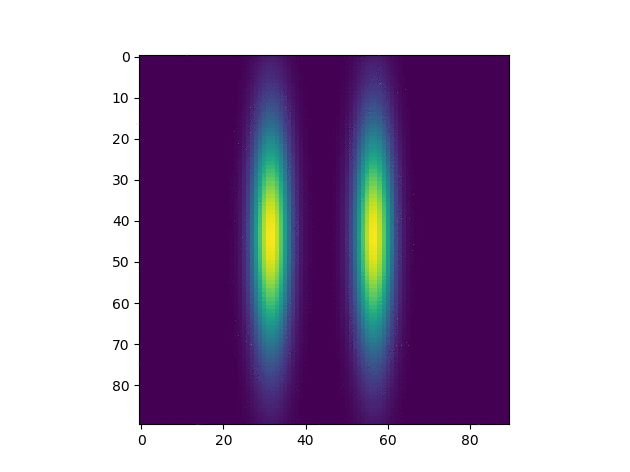
\includegraphics[width=\linewidth]{fig1.png}
            \caption{Two Gaussian distribution on a 2 dimensional matrix.}
            \label{gaussian}
        \end{subfigure}
        \begin{subfigure}[b]{0.4\linewidth}
            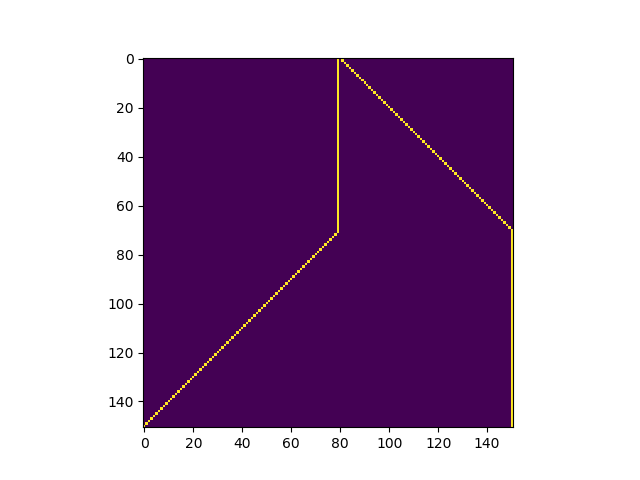
\includegraphics[width=\linewidth]{fig2.png}
            \caption{Shortest path in array with an obstacle in the middle.}
            \label{astar}
        \end{subfigure}
    \end{figure}



    \printbibliography{}
\end{document}